\documentclass{article}
\usepackage[utf8]{inputenc}
\usepackage[T1]{fontenc}
\usepackage[italian]{babel}
\usepackage{geometry}
\usepackage{graphicx}
\usepackage{amsmath}
\geometry{a4paper, margin=1in}

\title{Capitolo 3 - Crittografia Simmetrica e Confidenzialità}
\author{}
\date{}

\begin{document}

\maketitle

\noindent
La crittografia simmetrica, definita anche crittografia convenzionale, a chiave segreta o a chiave singola, era l'unico tipo di crittografia in uso prima dello sviluppo della crittografia a chiave pubblica alla fine degli anni '70. Rimane di gran lunga la più ampiamente utilizzata tra i due tipi di crittografia.

\begin{itemize}
    \item \textbf{Testo in chiaro:} Questo è il messaggio originale o i dati che vengono inseriti nell'algoritmo come input.
    \item \textbf{Algoritmo di crittografia:} L'algoritmo di crittografia esegue varie sostituzioni e trasformazioni sul testo in chiaro.
    \item \textbf{Chiave segreta:} La chiave segreta è anch'essa un input per l'algoritmo. Le esatte sostituzioni e trasformazioni eseguite dall'algoritmo dipendono dalla chiave.
    \item \textbf{Testo cifrato:} Questo è il messaggio rimescolato prodotto come output. Dipende dal testo in chiaro e dalla chiave segreta. Per un dato messaggio, due chiavi diverse produrranno due testi cifrati diversi.
    \item \textbf{Algoritmo di de-crittografia:} Questo è essenzialmente l'algoritmo di crittografia eseguito al contrario. Prende il testo cifrato e la stessa chiave segreta e produce il testo in chiaro originale.
\end{itemize}

I sistemi crittografici sono genericamente classificati secondo tre dimensioni indipendenti:

\begin{enumerate}
    \item \textbf{Il tipo di operazioni utilizzate per trasformare il testo in chiaro in testo cifrato.} Tutti gli algoritmi di crittografia si basano su due principi generali: la \textbf{sostituzione}, in cui ogni elemento del testo in chiaro (bit, lettera, gruppo di bit o lettere) viene mappato in un altro elemento, e la \textbf{trasposizione}, in cui gli elementi del testo in chiaro vengono riorganizzati. Il requisito fondamentale è che nessuna informazione vada persa (ovvero che tutte le operazioni siano reversibili).
    \item \textbf{Il numero di chiavi utilizzate.} Se sia il mittente che il ricevente utilizzano la stessa chiave, il sistema è definito simmetrico, a chiave singola, a chiave segreta o crittografia convenzionale. Se il mittente e il ricevente utilizzano ciascuno una chiave diversa, il sistema è definito asimmetrico, a due chiavi o crittografia a chiave pubblica.
    \item \textbf{Il modo in cui viene elaborato il testo in chiaro.} Un \textbf{cifrario a blocchi} elabora l'input un blocco di elementi alla volta, producendo un blocco di output per ogni blocco di input. Un \textbf{cifrario a flusso} elabora gli elementi di input continuamente, producendo un elemento di output alla volta, man mano che procede.
\end{enumerate}

\vspace{0.8cm}

\section*{Struttura della cifratura a blocchi - Cifrario di Feistel}

\begin{quote}
    \textit{Il cifrario a blocchi simmetrico consiste in una sequenza di cicli con sostituzioni e permutazioni controllate dalla chiave.}
\end{quote}

\noindent Questa regola è stata descritta per la prima volta da Horst Feistel nel 1973 quando propose il suo omonimo cifrario.

\vspace{0.5cm}

\noindent \begin{minipage}{0.45\textwidth}
    Gli input per l'algoritmo di crittografia sono un blocco di testo in chiaro di lunghezza 2w bit e una chiave K. Il blocco di testo in chiaro è diviso in due metà:
    
    \begin{equation*}
        L_0 \text{ e } R_0
    \end{equation*}
    
    Le due metà dei dati passano attraverso n round di elaborazione e poi si combinano per produrre il blocco di testo cifrato. Ogni round i ha come input:
    
    \begin{equation*}
        L_{i-1} \text{ e } R_{i-1}
    \end{equation*}
    
    derivati dal round precedente, così come una sottochiave:
    
    \begin{equation*}
        K_i
    \end{equation*}
    
    derivata dalla chiave complessiva K. In generale, le sotto-chiavi sono diverse da K e l'una dall'altra, e sono generate dalla chiave mediante un algoritmo di generazione delle sotto-chiavi.
\end{minipage}
\hfill
\begin{minipage}{0.5\textwidth}
    \centering
    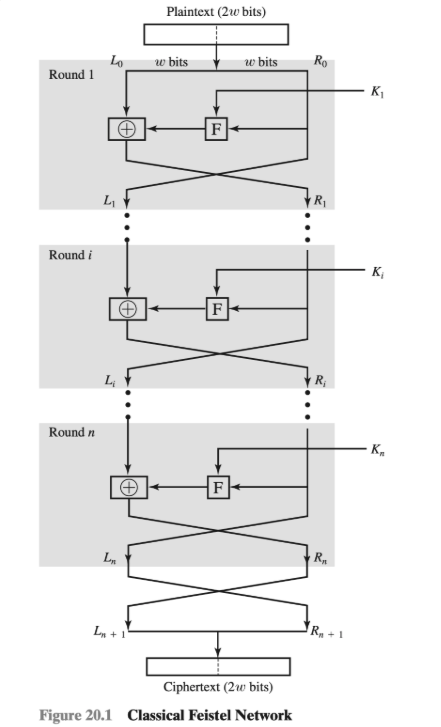
\includegraphics[width=\textwidth]{Screenshot 2026-04-29 alle 17.49.22.png}
\end{minipage}

\vspace{0.8cm}

Tutti i round hanno la stessa struttura. Viene eseguita una sostituzione sulla metà sinistra dei dati. Ciò avviene applicando una \textbf{funzione di round F} alla metà destra dei dati e prendendo poi l'OR esclusivo (XOR) dell'output di quella funzione e della metà sinistra dei dati. La funzione di round ha la stessa struttura generale per ogni round ma è parametrizzata dalla sottochiave di round $K_i$. In seguito a questa sostituzione, viene eseguita una permutazione che consiste nell'interscambio delle due metà dei dati. 

La struttura di Feistel è un esempio particolare della struttura più generale utilizzata da tutti i cifrari simmetrici a blocchi. In generale, un cifrario simmetrico a blocchi consiste in una sequenza di round, con ogni round che esegue sostituzioni e permutazioni condizionate da un valore di chiave segreta. L'esatta realizzazione di un cifrario simmetrico a blocchi dipende dalla scelta dei seguenti parametri e caratteristiche di progettazione:

\begin{itemize}
    \item \textbf{Dimensione del blocco:} Dimensioni del blocco più grandi significano maggiore sicurezza (a parità di altre condizioni) ma ridotta velocità di crittografia/decrittografia. Una dimensione del blocco di 128 bit è un compromesso ragionevole ed è quasi universale tra i recenti progetti di cifrari a blocchi.
    \item \textbf{Dimensione della chiave:} Una dimensione della chiave più grande significa maggiore sicurezza ma può diminuire la velocità di crittografia/decrittografia. La lunghezza della chiave più comune negli algoritmi moderni è 128 bit.
    \item \textbf{Numero di round:} L'essenza di un cifrario simmetrico a blocchi è che un singolo round offre una sicurezza inadeguata, ma che round multipli offrono una sicurezza crescente. Una dimensione tipica è 16 round.
    \item \textbf{Algoritmo di generazione delle sottochiavi:} Una maggiore complessità in questo algoritmo dovrebbe portare a una maggiore difficoltà della criptoanalisi.
    \item \textbf{Funzione di round:} Ancora una volta, una maggiore complessità significa generalmente una maggiore resistenza alla crittoanalisi.
\end{itemize}

\vspace{0.8cm}

\section*{Algoritmi di cifratura simmetrica}

Gli algoritmi di crittografia simmetrica più comunemente usati sono i cifrari a blocchi. Un cifrario a blocchi elabora l'input di testo in chiaro in blocchi di dimensione fissa e produce un blocco di testo cifrato di pari dimensione per ogni blocco di testo in chiaro. Questa sezione e la prossima si concentrano sui tre più importanti cifrari a blocchi simmetrici: il Data Encryption Standard (DES), il triple DES (3DES) e l'Advanced Encryption Standard (AES).

\vspace{0.5cm}

\subsection*{DES}

L'algoritmo DES ha un testo in chiaro è lungo 64 bit e la chiave è lunga 56 bit; quantità di testo in chiaro più lunghe vengono elaborate in blocchi da 64 bit. La struttura DES è una variante minore della rete di \textbf{Feistel}. Sono previsti 16 round di elaborazione. Nella fase di cifratura, dalla chiave originale a 56 bit vengono generate 16 \textbf{sottochiavi}, una delle quali viene utilizzata per ogni round. Il processo di \textbf{decrittografia} con DES è essenzialmente lo stesso del processo di crittografia. La regola è la seguente: utilizzare il testo cifrato come input per l'algoritmo DES, ma utilizzare le \textbf{sottochiavi} in ordine inverso.

\vspace{0.5cm}

\subsection*{Triple DES}

\vspace{0.2cm}
\noindent \begin{minipage}{0.48\textwidth}
    Il 3DES utilizza tre chiavi e tre esecuzioni dell'algoritmo DES. La funzione segue una sequenza \textbf{encrypt-decrypt-encrypt} (EDE):

    \begin{itemize}
        \item \textbf{Fase 1 (Criptazione):} Il testo in chiaro viene cifrato con la prima chiave (K1).
        \item \textbf{Fase 2 (Decriptazione):} Il risultato viene "decriptato" usando una seconda chiave (K2). Poiché K2 è diversa da K1, questa operazione non riporta al testo originale, ma crea un ulteriore livello di confusione (\textbf{scrambling}).
        \item \textbf{Fase 3 (Criptazione):} Il risultato viene cifrato un'ultima volta con la terza chiave (K3).
    \end{itemize}

    \vspace{0.3cm}
    La \textbf{decrittografia} è semplicemente la stessa operazione con le chiavi invertite.
\end{minipage}
\hfill
\begin{minipage}{0.48\textwidth}
    \centering
    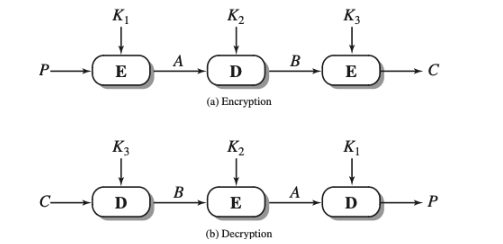
\includegraphics[width=\textwidth]{Screenshot 2026-04-29 alle 17.49.38.png}
    
    \vspace{0.5cm}
    \begin{equation*}
        C = E(K_3, D(K_2, E(K_1, P)))
    \end{equation*}
    \vspace{0.3cm}
    \begin{equation*}
        P = D(K_1, E(K_2, D(K_3, C)))
    \end{equation*}
\end{minipage}

\vspace{0.5cm}

Non vi è alcun significato crittografico nell'uso della \textbf{decrittografia} per la seconda fase della crittografia 3DES. Il suo unico vantaggio è che consente agli utenti del 3DES di \textbf{decrittografare} i dati \textbf{crittografati} dagli utenti del vecchio DES singolo.

\vspace{0.5cm}

\subsection*{AES}

È destinato a sostituire il DES e il triple DES con un algoritmo più sicuro ed efficiente. A differenza del DES, l'AES \textbf{non utilizza una struttura di Feistel}. Mentre i vecchi algoritmi dividevano il blocco a metà elaborandone solo una parte alla volta, l'AES elabora l'intero blocco di dati in parallelo.

\begin{itemize}
    \item \textbf{Dimensione del Blocco:} 128 bit (fissa).
    \item \textbf{Lunghezza della Chiave:} Può essere di 128, 192 o 256 bit.
    \item \textbf{Lo "State":} I dati vengono organizzati in una matrice quadrata 4x4 di byte chiamata \textbf{State}. Tutte le operazioni agiscono su questa "scacchiera" di 16 byte.
    \item \textbf{Iterazioni (Round):} Il numero di round dipende dalla chiave:
    \begin{itemize}
        \item 10 (per 128 bit)
        \item 12 (per 192 bit)
        \item 14 (per 256 bit).
    \end{itemize}
\end{itemize}

\vspace{0.5cm}

\subsubsection*{Rappresentazione dei Dati: Lo "State"}

I dati in input (128 bit) vengono organizzati in una \textbf{matrice quadrata 4x4 di byte} chiamata \textbf{State}. Tutte le trasformazioni dell'algoritmo operano su questa "scacchiera" di 16 byte. Anche la chiave viene visualizzata come una matrice di byte e poi espansa.

\vspace{0.5cm}

\subsubsection*{Espansione della Chiave}

L'algoritmo non usa la chiave originale così com'è in ogni round. La chiave iniziale (es. 128 bit) viene espansa in un array di 44 parole da 32 bit attraverso un algoritmo dedicato. Questo crea una \textbf{sotto-chiave unica per ogni round}, aumentando drasticamente la resistenza agli attacchi.

\vspace{0.8cm}

\subsubsection*{Le Quattro Fasi di un Round}

Ogni round (eccetto l'ultimo) applica quattro trasformazioni matematiche per garantire \textbf{confusione e diffusione}.

\vspace{0.5cm}

\noindent \textbf{1. Substitute Bytes (Sostituzione)}

\vspace{0.2cm}
\noindent \begin{minipage}{0.5\textwidth}
    Questa è una fase di sostituzione non lineare che opera indipendentemente su ogni byte dello \textit{State}.
    \begin{itemize}
        \item \textbf{Il Meccanismo:} Si utilizza una tabella di ricerca predefinita chiamata \textbf{S-box}, che consiste in una matrice 16x16 contenente una permutazione di tutti i possibili 256 valori a 8 bit.
        \item \textbf{Mappatura:} Per ogni byte, i 4 bit di sinistra (MSB) determinano la \textbf{riga} e i 4 bit di destra (LSB) determinano la \textbf{colonna} della S-box.
        \item \textbf{Esempio:} Se un byte ha valore esadecimale \textbf{\{95\}}, si incrocia la riga 9 con la colonna 5, ottenendo il valore \textbf{\{2A\}}.
        \item \textbf{Obiettivo:} È l'unica fase non lineare dell'AES. È progettata per avere una bassa correlazione tra bit di input e output, rendendo l'algoritmo resistente alla crittoanalisi statistica.
    \end{itemize}
\end{minipage}
\hfill
\begin{minipage}{0.45\textwidth}
    \centering
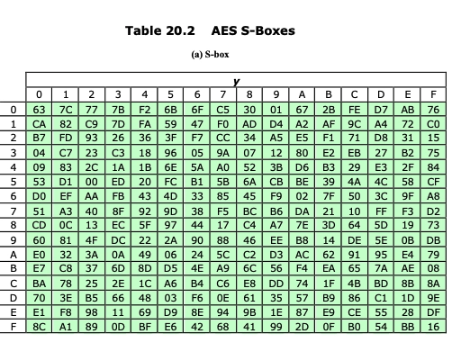
\includegraphics[width=\textwidth]{Screenshot 2026-04-29 alle 17.50.27.png}
\end{minipage}

\vspace{0.8cm}

\noindent \textbf{2. Shift Rows (Scorrimento Righe)}

\vspace{0.2cm}
\noindent \begin{minipage}{0.45\textwidth}
    Questa è una fase di permutazione che sposta i byte all'interno delle righe dello \textit{State}.
\end{minipage}
\hfill
\begin{minipage}{0.5\textwidth}
    \centering
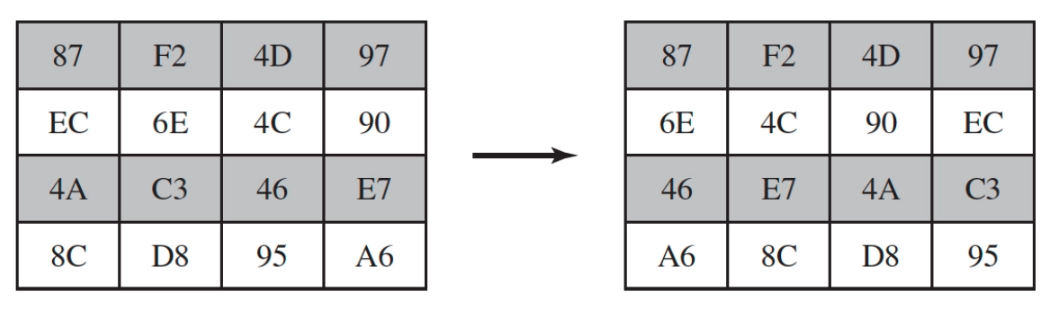
\includegraphics[width=\textwidth]{Screenshot 2026-04-29 alle 17.50.39.png}
\end{minipage}

\vspace{0.3cm}
\begin{itemize}
    \item \textbf{Procedimento:} Le righe della matrice vengono fatte scorrere circolarmente verso sinistra con offset differenti:
    \begin{itemize}
        \item \textbf{Riga 1:} Non subisce alcuna modifica.
        \item \textbf{Riga 2:} Scorrimento circolare a sinistra di \textbf{1 byte}.
        \item \textbf{Riga 3:} Scorrimento circolare a sinistra di \textbf{2 byte}.
        \item \textbf{Riga 4:} Scorrimento circolare a sinistra di \textbf{3 byte}.
    \end{itemize}
    \item \textbf{Impatto:} Questa trasformazione assicura che i quattro byte di una singola colonna vengano distribuiti in quattro colonne diverse per il round successivo.
    \item \textbf{Diffusione:} Sposta i dati tra le colonne, garantendo quella che i tuoi appunti chiamano "diffusione orizzontale".
\end{itemize}

\vspace{0.8cm}

\noindent \textbf{3. Mix Columns (Miscelazione colonne)}

\vspace{0.2cm}
\noindent \begin{minipage}{0.5\textwidth}
    Questa fase opera sulle colonne dello \textit{State}, trattando ogni colonna come un vettore matematico.
    \begin{itemize}
        \item \textbf{Il Calcolo:} Ogni byte di una colonna viene mappato in un nuovo valore che è funzione di \textbf{tutti e quattro} i byte della colonna stessa. Matematicamente, questo viene calcolato usando equazioni su \textbf{campi finiti}.
        \item \textbf{Proprietà:} È progettata per fornire un'ottima miscelazione dei bit.
        \item \textbf{Diffusione Totale:} Combinata con lo \textit{Shift Rows}, garantisce che dopo pochi round ogni bit di output dipenda potenzialmente da ogni singolo bit di input (effetto valanga).
    \end{itemize}
\end{minipage}
\hfill
\begin{minipage}{0.45\textwidth}
    \centering
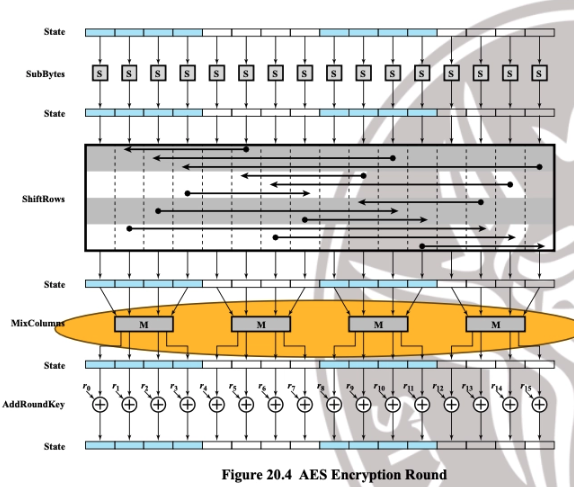
\includegraphics[width=\textwidth]{Screenshot 2026-04-29 alle 17.50.57.png}
    
    \vspace{0.3cm}
    \begin{itemize}
        \item \textbf{Eccezione: Questa fase non viene eseguita} nell'ultimo round (il decimo round per AES-128) per rendere il cifrario correttamente reversibile durante la decrittazione.
    \end{itemize}
\end{minipage}

\vspace{0.8cm}

\noindent \textbf{4. Add Round Key (Aggiunta Chiave)}

\vspace{0.2cm}
\noindent \begin{minipage}{0.5\textwidth}
    È l'operazione più semplice ma la più cruciale, poiché è l'unica che introduce la segretezza della chiave.
    \begin{itemize}
        \item \textbf{Operazione:} Viene eseguito un \textbf{XOR bit a bit} tra i 128 bit dello \textit{State} e i 128 bit della chiave di round corrente.
        \item \textbf{Flessibilità:} Può essere vista come un'operazione colonna per colonna (ogni colonna dello stato contro una parola della chiave) o come una semplice operazione a livello di byte.
        \item \textbf{Inversione:} Per decifrare, si esegue nuovamente lo XOR con la stessa chiave di round, poiché l'operazione XOR è l'inversa di se stessa ($A \oplus B \oplus B = A$).
    \end{itemize}
\end{minipage}
\hfill
\begin{minipage}{0.45\textwidth}
    \centering
    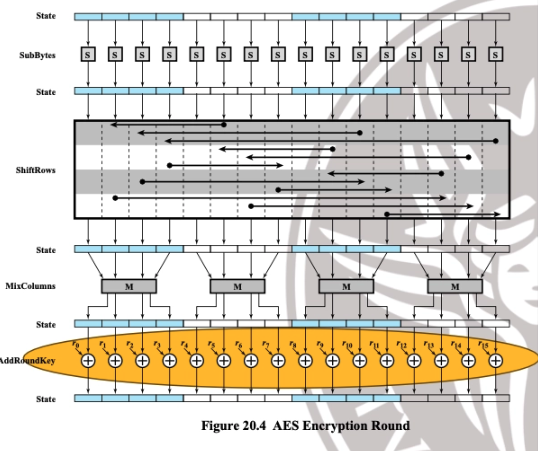
\includegraphics[width=\textwidth]{Screenshot 2026-04-29 alle 17.51.37.png}
    
    \vspace{0.3cm}
    \begin{itemize}
        \item \textbf{Posizionamento:} Il cifrario inizia e finisce sempre con questa fase. Qualsiasi altra fase all'inizio o alla fine sarebbe inutile, poiché invertibile senza conoscere la chiave.
    \end{itemize}
\end{minipage}

\vspace{0.8cm}

\subsubsection*{Sequenza del Cifrario}

L'algoritmo segue questa struttura specifica:

\begin{enumerate}
    \item \textbf{Inizio:} Fase preliminare di \textit{Add Round Key}.
    \item \textbf{Corpo:} 9 round completi (tutte e 4 le fasi).
    \item \textbf{Conclusione:} Un 10° round che \textbf{salta il Mix Columns} e termina con l'ultimo \textit{Add Round Key}.
\end{enumerate}

\vspace{0.8cm}

\section*{Struttura della cifratura a flusso}

\begin{quote}
    \textit{A differenza dei cifrari a blocco, un cifrario a flusso elabora gli elementi dell'input (bit, byte o parole) in modo \textbf{continuo}.}
\end{quote}

Un generatore di bit \textbf{pseudocasuali} prende una chiave in input e produce uno stream di numeri simili a quelli casuali (\textbf{keystream}). Lo stream generato deve essere imprevedibile senza la conoscenza della chiave di input. Per effettuare le operazioni di cifratura e decrittazione, si esegue un'operazione \textbf{XOR} tra lo stream di byte del testo in chiaro (M) e lo stream di chiavi (k) per ottenere il testo cifrato (C). Il processo è identico per la decrittazione.

\vspace{0.8cm}

\section*{Algoritmo RC4}

L'RC4 è un cifrario a flusso a dimensione di chiave variabile con operazioni orientate ai byte. Si basa sull'uso di una permutazione casuale ed è noto per la sua semplicità e velocità (richiede da 8 a 16 operazioni macchina per ogni byte di output). Presenta due fasi:

\subsection*{Fase di Inizializzazione}

L'algoritmo inizia preparando uno stato interno tramite una chiave di lunghezza variabile (da 1 a 256 byte):

\begin{itemize}
    \item \textbf{Vettore di Stato S:} Viene inizializzato un vettore S di 256 byte con elementi da 0 a 255 ($S[0]=0, S[1]=1, \dots, S[255]=255$).
    \item \textbf{Vettore Temporaneo T:} Se la chiave K è lunga 256 byte, viene copiata in T. Se è più corta, viene ripetuta ciclicamente fino a riempire i 256 byte di T.
    \item \textbf{Permutazione Iniziale:} Si scorre il vettore S scambiando ogni elemento S[i] con un altro elemento S[j] secondo uno schema dettato da T:
\end{itemize}

\begin{equation*}
    j = (j + S[i] + T[i]) \pmod{256}
\end{equation*}

\begin{equation*}
    Swap(S[i], S[j])
\end{equation*}

\begin{itemize}
    \item Dopo questa fase, il vettore S contiene ancora tutti i numeri da 0 a 255, ma permutati casualmente; la chiave originale non viene più utilizzata.
\end{itemize}

\subsection*{Generazione dello Stream}

Una volta inizializzato S, l'algoritmo genera un byte di chiave k alla volta:

\begin{enumerate}
    \item Si incrementa i e si calcola j basandosi sui valori correnti di S:
    \begin{equation*}
        i = (i + 1) \pmod{256}
    \end{equation*}
    \begin{equation*}
        j = (j + S[i]) \pmod{256}
    \end{equation*}
    \item Si scambiano nuovamente S[i] e S[j].
    \item Si calcola l'indice t per estrarre il byte dello stream k:
    \begin{equation*}
        t = (S[i] + S[j]) \pmod{256}
    \end{equation*}
    \begin{equation*}
        k = S[t]
    \end{equation*}
\end{enumerate}

\noindent \textbf{Cifratura:} Il valore k viene XORato con il byte di testo in chiaro.

\noindent \textbf{Decrittazione:} Il valore k viene XORato con il byte di testo cifrato.

\vspace{0.8cm}

\section*{Modalità di Funzionamento (Block Cipher Modes)}

Le modalità di funzionamento definiscono come applicare algoritmi come l'AES a messaggi più lunghi di un singolo blocco.

\subsection*{Modalità Electronic Codebook (ECB)}

Il modo più semplice per procedere è quello noto come modalità \textbf{electronic codebook (ECB)}, in cui il testo in chiaro viene gestito b bit alla volta e ogni blocco di testo in chiaro viene cifrato utilizzando la stessa chiave. Il termine \textbf{codebook} (libro dei codici) viene utilizzato perché, per una data chiave, esiste un testo cifrato unico per ogni blocco di testo in chiaro da b bit. Pertanto, si può immaginare un gigantesco libro dei codici in cui è presente una voce per ogni possibile pattern di testo in chiaro da b bit che mostra il corrispondente testo cifrato.

Con l'ECB, se lo stesso blocco da b bit appare più di una volta nel messaggio, produce sempre lo stesso testo cifrato. Per questo motivo, per messaggi lunghi, la modalità ECB potrebbe non essere sicura. Se il messaggio è altamente strutturato, potrebbe essere possibile per un \textbf{crittoanalista} sfruttare queste regolarità. Ad esempio, se è noto che il messaggio inizia sempre con determinati campi predefiniti, il \textbf{crittoanalista} potrebbe avere un numero di coppie testo in chiaro-testo cifrato note con cui lavorare. Se il messaggio presenta elementi ripetitivi, con un periodo di ripetizione multiplo di b bit, questi elementi possono essere identificati dall'analista. Ciò può aiutare nell'analisi o fornire l'opportunità di sostituire o riorganizzare i blocchi.

Per superare le carenze di sicurezza dell'ECB, vorremmo una tecnica in cui lo stesso blocco di testo in chiaro, se ripetuto, produca blocchi di testo cifrato diversi.

\subsection*{Modalità Cipher Block Chaining (CBC)}

Nella modalità \textbf{cipher block chaining (CBC)}, l'input dell'algoritmo di cifratura è lo XOR del blocco di testo in chiaro corrente e del testo cifrato precedente.

\vspace{0.2cm}
\noindent \begin{minipage}{0.48\textwidth}
    Viene utilizzata la stessa chiave per ogni blocco. In effetti, abbiamo "incatenato" insieme l'elaborazione della sequenza di blocchi di testo in chiaro. L'input della funzione di cifratura per ogni blocco di testo in chiaro non ha una relazione fissa con il blocco di testo in chiaro stesso. Pertanto, i pattern ripetuti di b bit non vengono esposti.
\end{minipage}
\hfill
\begin{minipage}{0.48\textwidth}
    \centering
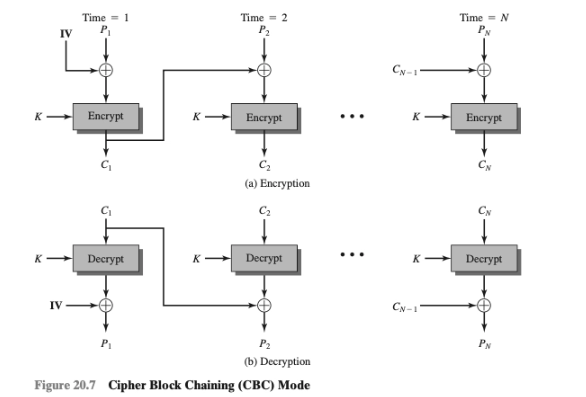
\includegraphics[width=\textwidth]{Screenshot 2026-04-29 alle 17.51.53.png}
\end{minipage}

\vspace{0.5cm}

Per la decrittazione, ogni blocco cifrato viene fatto passare attraverso l'algoritmo di decrittazione. Il risultato viene sottoposto a XOR con il blocco di testo cifrato precedente per produrre il blocco di testo in chiaro. Per vedere come funziona, possiamo scrivere:

\begin{equation*}
    C_j = E(K, [C_{j-1} \oplus P_j])
\end{equation*}

\noindent dove $E(K,X)$ è la cifratura del testo in chiaro X utilizzando la chiave K, e $\oplus$ è l'operazione di OR esclusivo (XOR). Allora:

\begin{align*}
    D(K, C_j) &= D(K, E(K, [C_{j-1} \oplus P_j])) \\
    D(K, C_j) &= C_{j-1} \oplus P_j \\
    C_{j-1} \oplus D(K, C_j) &= C_{j-1} \oplus C_{j-1} \oplus P_j = P_j
\end{align*}

\noindent il che verifica il processo di decrittazione.

Per produrre il primo blocco di testo cifrato, un \textbf{vettore di inizializzazione (IV)} viene sottoposto a XOR con il primo blocco di testo in chiaro. In decrittazione, l'IV viene sottoposto a XOR con l'output dell'algoritmo di decrittazione per recuperare il primo blocco di testo in chiaro. L'IV deve essere noto sia al mittente che al ricevente. Per la massima sicurezza, l'IV dovrebbe essere protetto così come la chiave. Questo potrebbe essere fatto inviando l'IV tramite cifratura ECB.

Una ragione per proteggere l'IV è la seguente: se un avversario è in grado di ingannare il ricevente spingendolo a usare un valore diverso per l'IV, allora l'avversario è in grado di invertire bit selezionati nel primo blocco di testo in chiaro. Per vederlo, considera quanto segue:

\begin{align*}
    C_1 &= E(K, [IV \oplus P_1]) \\
    P_1 &= IV \oplus D(K, C_1)
\end{align*}

\noindent Sia X[i] il i-esimo bit della quantità da b bit X. Allora:

\begin{equation*}
    P_1[i] = IV[i] \oplus D(K, C_1)[i]
\end{equation*}

\noindent Quindi, usando le proprietà dello XOR, possiamo affermare:

\begin{equation*}
    P_1[i]' = IV[i]' \oplus D(K, C_1)[i]
\end{equation*}

\noindent dove la notazione "primo" (') indica la \textbf{complementazione} del bit (inversione). Ciò significa che se un avversario può cambiare i bit nell'IV in modo prevedibile, i bit corrispondenti del valore ricevuto di P1 possono essere modificati.

\subsection*{Modalità Cipher Feedback (CFB)}

È possibile convertire qualsiasi cifrario a blocchi in un \textbf{cifrario a flusso} utilizzando la modalità \textbf{cipher feedback (CFB)}. Un cifrario a flusso elimina la necessità di completare (\textbf{padding}) un messaggio per renderlo un numero intero di blocchi. Può anche operare in tempo reale. Pertanto, se viene trasmesso un flusso di caratteri, ogni carattere può essere cifrato e trasmesso immediatamente utilizzando un cifrario a flusso orientato ai caratteri.

\vspace{0.2cm}
\noindent \begin{minipage}{0.48\textwidth}
    Una proprietà desiderabile di un cifrario a flusso è che il testo cifrato sia della stessa lunghezza del testo in chiaro. Quindi, se vengono trasmessi caratteri a 8 bit, ogni carattere dovrebbe essere cifrato utilizzando 8 bit. Se si utilizzano più di 8 bit, la capacità di trasmissione viene sprecata.
    
    Nello schema CFB, si assume che l'unità di trasmissione sia di s bit; un valore comune è s=8. Come nel CBC, le unità di testo in chiaro sono concatenate tra loro, in modo che il testo cifrato di qualsiasi unità di testo in chiaro sia una funzione di tutto il testo in chiaro precedente.
\end{minipage}
\hfill
\begin{minipage}{0.48\textwidth}
    \centering
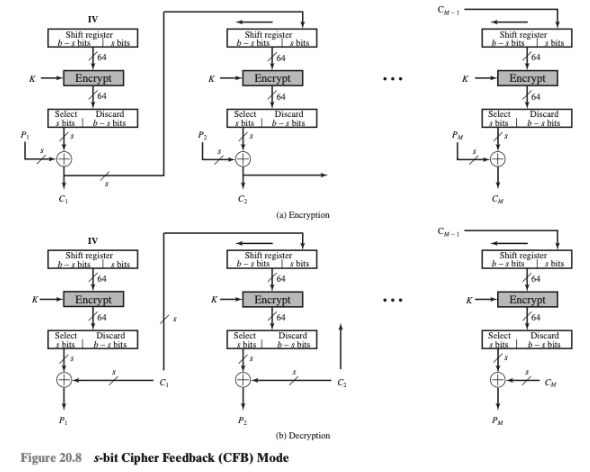
\includegraphics[width=\textwidth]{Screenshot 2026-04-29 alle 17.52.05.png}
\end{minipage}

\vspace{0.5cm}

Consideriamo prima la cifratura. L'input della funzione di cifratura è uno \textbf{shift register} da b bit impostato inizialmente su un vettore di inizializzazione (IV). Gli s bit più significativi (a sinistra) dell'output della funzione di cifratura vengono sottoposti a XOR con la prima unità di testo in chiaro P1 per produrre la prima unità di testo cifrato C1, che viene quindi trasmessa. Inoltre, il contenuto dello \textbf{shift register} viene spostato a sinistra di s bit e C1 viene inserito negli s bit più a destra (meno significativi) dello \textbf{shift register}. Questo processo continua finché tutte le unità di testo in chiaro non sono state cifrate.

Per la decrittazione viene utilizzato lo stesso schema, tranne per il fatto che l'unità di testo cifrato ricevuta viene sottoposta a XOR con l'output della funzione di cifratura per produrre l'unità di testo in chiaro. Si noti che viene utilizzata la funzione di \textbf{cifratura} (encryption) e non quella di decrittazione.

\subsection*{Modalità Counter (CTR)}

Sebbene l'interesse per la modalità \textbf{counter} (CTR) sia aumentato recentemente con applicazioni alla sicurezza delle reti ATM e IPsec, questa modalità è stata proposta molto presto.

Viene utilizzato un contatore di dimensione pari a quella del blocco di testo in chiaro. L'unico requisito stabilito dallo standard SP 800-38A è che il valore del contatore deve essere diverso per ogni blocco di testo in chiaro cifrato. Tipicamente, il contatore viene inizializzato a un certo valore e poi incrementato di 1 per ogni blocco successivo (modulo $2^b$, dove b è la dimensione del blocco). Per la cifratura, il contatore viene cifrato e poi sottoposto a XOR con il blocco di testo in chiaro per produrre il blocco di testo cifrato; non c'è concatenamento. Per la decrittazione, viene utilizzata la stessa sequenza di valori del contatore, con ogni contatore cifrato sottoposto a XOR con un blocco di testo cifrato per recuperare il blocco di testo in chiaro corrispondente.

\end{document}